\chapter{Algebraic Diagrammatic Construction (ADC)}

The \ac{ADC} is a Green's function approach for the calculation of ionization
nergies and electron affinities.
Its advantage is the ability to determine the desired ionization energies
without explicit calculation of the initial and final states, but instead
obtaining their energy differences directly.

Originally, the Green's function was formulated in the Dyson ansatz and
determined using perturbation theory. This way both the ionization and the
electron affinity part had to be included in the description. In the non-Dyson
scheme those two are separable and hence the dimension of the problem is reduced
when one is interested in either the $N+1$ or the $N-1$ part \cite{Schirmer98}.

\begin{equation}
 G_{pq}(\omega) = G^+_{pq}(\omega) + G^-_{pq}(\omega)
\end{equation}

The ionization part $\mathbf{G^-}(\omega)$ is transposed to give
$\tilde{G}_{pq}(\omega) = G^-_{qp}(\omega)$. From this, the compact matrix
form can be deduced

\begin{equation}\label{matrixspec}
\mathbf{\tilde{G}}(\omega) = \mathbf{x}^\dagger(\omega-\mathbf{\Omega})^{-1}\mathbf{x}
\end{equation}

To this point, the approach is exact. However, the exact wavefunctions are unknown
and hence the basis of so-called \emph{intermediate states} is introduced. These
are formally constructed from \ac{CES} as they appear in a
\ac{CI} expansion. These \ac{CES} are then grouped into excitation classes
and these classes are orthogonalized with respect to each other. Afterwards,
the states within each class are orthogonalized. 
This approach has the advantage to be size-consistent and hence
suiTable for the description of larger systems. \cite{Mertins96_1}

In this \ac{ISR} the Green's function can be written as
\begin{equation}\label{isradc}
\mathbf{\tilde{G}}(\omega) = \mathbf{f}^\dagger(\omega-\mathbf{M})^{-1}\mathbf{f}
\end{equation}

with the Hamiltonian $\mathbf{M}$.
This equation can be solved by
considering the eigenvalue problem

\begin{equation}\label{adcewp}
(\mathbf{K}+\mathbf{C}) \mathbf{Y} = \mathbf{Y}\mathbf{\Omega} \quad\text{where } \mathbf{Y}^\dagger\mathbf{Y}=\mathbf{1}
\end{equation}
where $\mathbf{\Omega}$ is the matrix of eigenvalues and hence the ionization
energies and $\mathbf{Y}$ is the matrix of eigenvectors which connects the
intermediate state representation with the exact $N-1$ solutions.

\begin{equation}
 \mathbf{x} = \mathbf{Y}^\dagger \mathbf{f}
\end{equation}

For the construction of the \ac{ADC} matrix $\mathbf{M}$ and the
effective transitions moments $\mathbf{f}$, $\mathbf{M}$ and $\mathbf{f}$
are expanded into different orders of perturbations and inserted to equation
(\ref{isradc}).

\begin{eqnarray}
\mathbf{M} &=& \mathbf{M}^{(0)} + \mathbf{M}^{(1)} + \mathbf{M}^{(2)} + \cdots\label{stf}\\
\mathbf{f} &=& \mathbf{f}^{(0)} + \mathbf{f}^{(1)} + \mathbf{f}^{(2)} + \cdots\label{stf}
\end{eqnarray}

From this, different orders of perturbation theory of the Hamiltonian can be
constructed successively. Hereby, the truncation after the $n$-th order leads
to ADC($n$). The contributions to the different classes for different
orders of \ac{ADC} are shown
in Figure \ref{figure:adcmat_pgf}.

\begin{figure}[h]
  \centering
  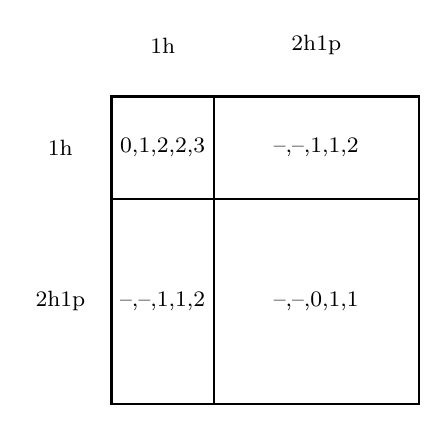
\begin{tikzpicture}[scale=1.3]
    \footnotesize
    %\draw [help lines] (-1,0) grid (23,5);
    \draw [thick] (0,0) rectangle (3,3);
    \draw [thick] (0,2) rectangle (1,3) node [midway] {0,1,2,2,3};
    \draw [thick] (1,0) rectangle (3,2) node [midway] {--,--,0,1,1};
    \draw [thick] (0,0) rectangle (1,2) node [midway] {--,--,1,1,2};
    \draw [thick] (1,2) rectangle (3,3) node [midway] {--,--,1,1,2};
    \node (1h1) at (0.5,3.5) {1h};
    \node (1h2) at (-0.5,2.5) {1h};
    \node (2h1) at (2.0,3.5) {2h1p};
    \node (2h2) at (-0.5,1.0) {2h1p};

\end{tikzpicture}

  \caption{Schematic illustration of an \ac{ADC}($n$) matrix for different orders
           of perturbation for $n=0,1,2,2x,3$. ADC(2x) is an extended ADC(2)
           including first
           order contributions to the satellite block.}
  \label{figure:adcmat_pgf}
\end{figure}

The matrix elements of ADC(2x) are explicitely given by
\begin{itemize}
 \item 1h/1h (1h block):
   \begin{align}
    M_{kk'}^{(0)} &= \varepsilon_k \delta_{kk'} \\
    M_{kk'}^{(1)} &= 0 \\
    M_{kk'}^{(2)} &= -\frac12 \sum\limits_{abl} V_{ab[kl]} V_{k'l[ab]} %\times
                     \frac{\varepsilon_a+\varepsilon_b-\varepsilon_l
                       -\frac12 \varepsilon_k-\frac12 \varepsilon_{k'}}
                     {(\varepsilon_a+\varepsilon_b-\varepsilon_k-\varepsilon_l)
                      (\varepsilon_a+\varepsilon_b-\varepsilon_{k'}-\varepsilon_l)}
   \end{align}
 \item 1h/2h1p (coupling block):
   \begin{equation}
    M_{j,akl}^{(1)} = V_{kl[aj]}
   \end{equation}
 \item 2h1p/2h1p (satellite block):
   \begin{align}
    M_{akl,a'k'l'}^{(0)} &= (-\varepsilon_a+\varepsilon_k+\varepsilon_l)
                             \, \delta_{aa'}\delta_{kk'}\delta_{ll'} \\
    M_{akl,a'k'l'}^{(1)} &= -\delta_{aa'} V_{k'l'[kl]} + \delta_{kk'} V_{al'[a'l]}
                            +\delta_{ll'} V_{ak'[a'k]} - (k \leftrightarrow l)
   \end{align}
\end{itemize}

Here, $\varepsilon$ denotes the Hartree Fock energy. The occupied states are labelled
by $i,j,k,\dots$ and the unoccupied states are labelled by $a,b,c,\dots$. The
two-electron integrals for any combination of occupied and unoccupied orbitals
labelled by $p,q,r,s$ read as
\begin{equation}
 V_{pqrs} = \braket{\varphi_p(1)\varphi_q(2) |V(1,2)| \varphi_r(1)\varphi_s(2)}
\end{equation}

and $V_{pq[rs]} = V_{pqrs} - V_{pqsr}$.

